\section{Huấn luyện CLIP}

\begin{frame}{3.3 Huấn luyện CLIP}
    \begin{enumerate}
        \item Tiền xử lý dữ liệu
        \item Chuẩn bị Batch dữ liệu và mã hóa
        \item Mã hóa song song
        \item Tính toán ma trận tương đồng Cosine
        \item Hàm mất mát
        \item Tối ưu hóa
    \end{enumerate}
\end{frame}

% \begin{frame}{4.1 Phân tích dữ liệu huấn luyện}
%     CLIP không chỉ dựa vào kiến trúc mô hình thông minh mà còn nhờ vào bộ dữ liệu WIT (WebImageText) khổng lồ và đa dạng.

%     \begin{block}{Bộ dữ liệu WIT (WebImageText) - Trái tim của CLIP}
%         \begin{itemize}
%             \item \textbf{Quy mô:} Hơn 400 triệu cặp (hình ảnh, văn bản) thu thập từ internet.
%             \item \textbf{Đa dạng:} Bao phủ một lượng lớn các khái niệm, đối tượng, hành động, phong cách nghệ thuật, và ngữ cảnh khác nhau. Đây là yếu tố then chốt cho khả năng "zero-shot".
%             \item \textbf{Tính "nhiễu" (Noisy):} Dữ liệu từ internet không được gán nhãn thủ công một cách hoàn hảo. Văn bản đi kèm có thể không hoàn toàn mô tả chính xác hình ảnh.
%             \item \textbf{Chiến lược lọc:} Một số truy vấn cơ bản được sử dụng để thu thập dữ liệu. Lọc bỏ các truy vấn quá phổ biến hoặc không phù hợp.
%         \end{itemize}
%     \end{block}
% \end{frame}

% \begin{frame}
%     \textbf{Tại sao dữ liệu "nhiễu" và đa dạng lại quan trọng?}
%     \begin{itemize}
%         \item \textbf{Khả năng khái quát hóa:} Học từ dữ liệu đa dạng giúp mô hình không bị "overfit" vào một tập khái niệm hẹp.
%         \item \textbf{Robustness:} Sự "nhiễu" trong dữ liệu huấn luyện khiến mô hình trở nên mạnh mẽ hơn trước các biến thể và sự không hoàn hảo của dữ liệu thực tế.
%         \item \textbf{Hiệu quả về chi phí:} Thu thập dữ liệu quy mô lớn từ web rẻ hơn nhiều so với việc gán nhãn thủ công hàng trăm triệu mẫu.
%     \end{itemize} 
% \end{frame}


% \begin{frame}{4.2 Kiến trúc mô hình CLIP}
%     CLIP có kiến trúc hai nhánh (dual encoder):
%     \begin{itemize}
%         \item \textbf{Bộ mã hóa ảnh:} ResNet hoặc Vision Transformer (ViT), tạo ra vector đặc trưng cho ảnh.
%         \item \textbf{Bộ mã hóa văn bản:} Một Transformer nhẹ, mã hóa caption thành vector.
%     \end{itemize}
%     \bigskip
    
%     Hai encoder ánh xạ ảnh và văn bản vào cùng một không gian embedding sao cho các cặp khớp gần nhau, và cặp không khớp thì xa nhau.
    
%     \textbf{Phương pháp huấn luyện:}
%     \begin{itemize}
%         \item Dựa trên \textit{contrastive learning}, sử dụng hàm mất mát InfoNCE đối xứng.
%         \item Ma trận cosine similarity được tính giữa tất cả ảnh–văn bản trong minibatch.
%         \item Dùng hệ số nhiệt (\textit{temperature}) để điều chỉnh phân bố softmax.
%     \end{itemize}
% \end{frame}

\begin{frame}{3.3 Huấn luyện CLIP}
%    Quá trình huấn luyện CLIP tập trung vào việc học một không gian nhúng %    (embedding space) đa phương thức hiệu quả.
    \textbf{1. Tiền xử lý dữ liệu:}
    \begin{itemize}
        \item \textbf{Tiền xử lý ảnh:} Resize, crop ngẫu nhiên, chuẩn hóa theo ImageNet.
        \item \textbf{Tiền xử lý văn bản:} Token hóa bằng BPE, padding cho đồng đều độ dài.
    \end{itemize}
    \bigskip
    
    \textbf{2. Chuẩn bị Batch dữ liệu và mã hóa:}
    \begin{itemize}
        \item Một batch gồm N cặp (hình ảnh, văn bản) thực tế từ bộ dữ liệu WIT.
        \item Ví dụ: (I$_1$, T$_1$), (I$_2$, T$_2$), ..., (I$_N$, T$_N$).
    \end{itemize}
\end{frame}

\begin{frame}{3.3 Huấn luyện CLIP}
    \textbf{3. Mã hóa song song:}
    \begin{itemize}
        \item \textbf{Image Encoder (ResNet/ViT):} Mã hóa N hình ảnh thành N vector đặc trưng hình ảnh: $E_I = [e_{I1}, e_{I2}, ..., e_{IN}]$.
        \item \textbf{Text Encoder (Transformer):} Mã hóa N văn bản thành N vector đặc trưng văn bản: $E_T = [e_{T1}, e_{T2}, ..., e_{TN}]$.
        \item Các vector được chiếu (projected) vào cùng một không gian nhúng và chuẩn hóa L2.
    \end{itemize}
    \bigskip

    \textbf{4. Tính toán ma trận tương đồng Cosine:}
    \begin{itemize}
        \item Tạo ma trận N x N, trong đó phần tử (i, j) là độ tương đồng cosine giữa $e_{Ii}$ và $e_{Tj}$.
        \item Các phần tử trên đường chéo chính (i=j) đại diện cho các cặp (hình ảnh, văn bản) "đúng" (positive pairs).
        \item N$^2$ - N phần tử còn lại là các cặp "sai" (negative pairs).
    \end{itemize}
\end{frame}

\begin{frame}{}
    \begin{figure}
        \centering
        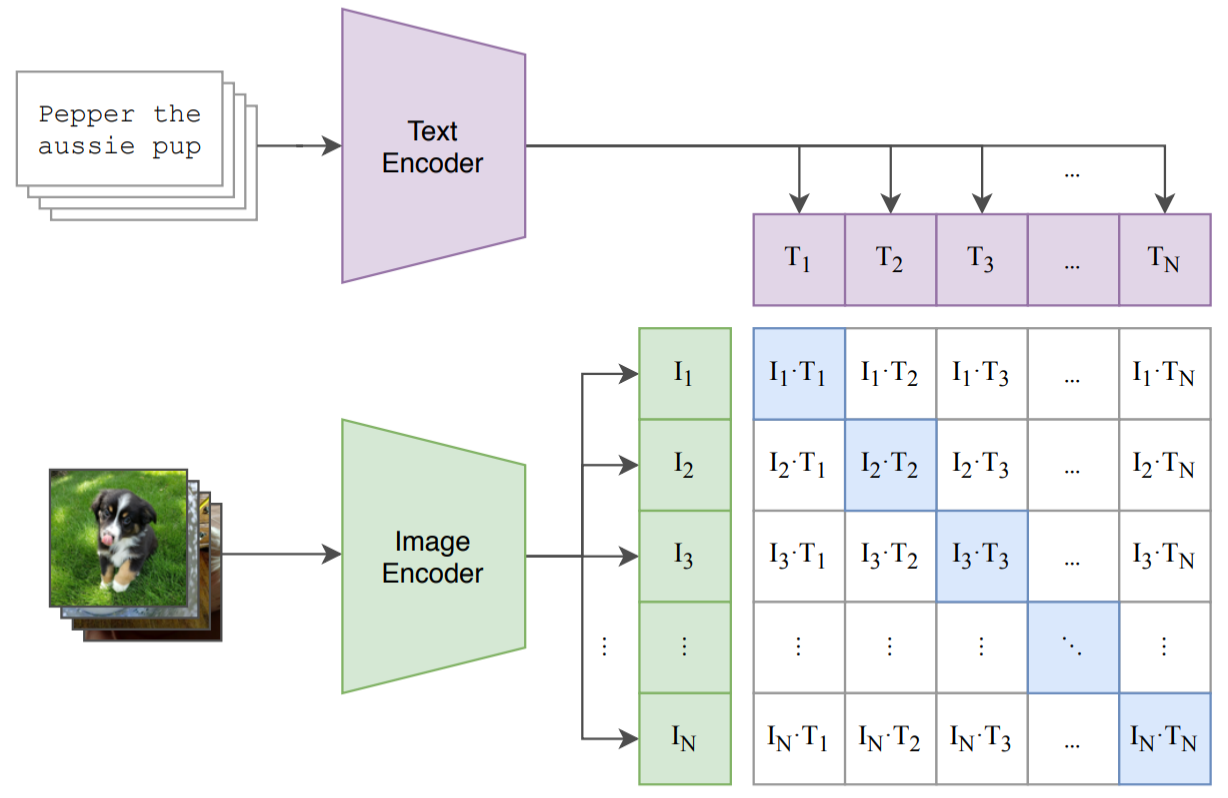
\includegraphics[width=0.8\linewidth]{img/01-similarity_matrix.png}
    \end{figure}
\end{frame}

\begin{frame}{3.3 Huấn luyện CLIP}
    \textbf{5. Hàm mất mát (Symmetric Cross-Entropy Loss):}
    \begin{itemize}
        \item Mục tiêu: Tối đa hóa độ tương đồng của các cặp "đúng" và tối thiểu hóa độ tương đồng của các cặp "sai".
        \item Tính toán loss cho cả hai chiều: image-to-text và text-to-image.
        \item $\mathcal{L}_{\text{i2t}} = -\sum_{i=1}^{N} \log \frac{\exp(S_{ii}/\tau)}{\sum_{j=1}^{N} \exp(S_{ij}/\tau)}$
        \item $\mathcal{L}_{\text{t2i}} = -\sum_{j=1}^{N} \log \frac{\exp(S_{jj}/\tau)}{\sum_{i=1}^{N} \exp(S_{ij}/\tau)}$
        \item Loss tổng: $(\mathcal{L}_{\text{i2t}} + \mathcal{L}_{\text{t2i}})/2$.
        \item $\tau$ là tham số nhiệt độ (temperature parameter) có thể học được, điều chỉnh độ "sắc nét" của phân phối xác suất.
    \end{itemize}

    \textbf{6. Tối ưu hóa:}
    \begin{itemize}
        \item Sử dụng optimizer AdamW.
        \item Batch size rất lớn (ví dụ: 32,768) để có đủ lượng mẫu negative hiệu quả.
        \item Huấn luyện hỗn hợp chính xác (mixed-precision training) để tăng tốc và giảm bộ nhớ.
    \end{itemize}
\end{frame}

\begin{frame}{3.4 Multi-modal Embedding Space - Sản phẩm cốt lõi}
    \begin{itemize}
        \item \textbf{Không gian thống nhất:} Một không gian vector cao chiều nơi biểu diễn của hình ảnh và văn bản có thể được so sánh trực tiếp.
        \item \textbf{Phản ánh mối quan hệ ngữ nghĩa:}
        \begin{itemize}
            \item Các cặp có mối quan hệ sẽ có các vector nằm rất gần nhau (độ tương đồng cosine cao).
            \item Các cặp không liên quan  sẽ có các vector nằm xa nhau (độ tương đồng cosine thấp).
        \end{itemize}
        \item \textbf{Khả năng "Open-set":} Vì được học từ dữ liệu ngôn ngữ tự nhiên đa dạng (WIT), không bị giới hạn bởi các lớp cố định. Có thể hiểu các khái niệm chưa từng thấy trong huấn luyện nếu có mô tả bằng ngôn ngữ tương ứng.
    \end{itemize}
\end{frame}

\begin{frame}{4.1 So sánh các mô hình biến thể CLIP}
    CLIP được huấn luyện với nhiều kiến trúc Image Encoder và kích thước khác nhau, dẫn đến các biến thể với hiệu suất và chi phí tính toán khác nhau.

    \begin{block}{Các biến thể chính và hiệu suất Zero-Shot trên ImageNet}
        \begin{itemize}
            \item \textbf{ResNet-50:} Độ chính xác 59.6\% (baseline)
            \item \textbf{ResNet-101:} Độ chính xác 62.2\%
            \item \textbf{ResNet-50x4 (scaled ResNet):} Độ chính xác 65.8\%
            \item \textbf{ViT-B/32 (Vision Transformer - Base, patch size 32):} Độ chính xác 63.2\%
            \item \textbf{ViT-B/16:} Độ chính xác 68.6\%
            \item \textbf{ViT-L/14 (Vision Transformer - Large, patch size 14):} Độ chính xác 75.3\%
            \item \textbf{ViT-L/14@336px (fine-tuned với độ phân giải cao hơn):} Độ chính xác 76.2\%
        \end{itemize}
    \end{block}
\end{frame}

\begin{frame}{4.2 Ưu điểm và hạn chế của CLIP}
    \begin{columns}[T]
        \begin{column}{0.5\textwidth}
            \begin{block}{Ưu điểm nổi bật}
                \begin{itemize}
                    \item Khả năng Zero-Shot mạnh mẽ.
                    \item Học từ dữ liệu web tự nhiên.
                    \item Mô hình nền tảng (Foundation Model).
                    \item Robustness.
                \end{itemize}
            \end{block}
        \end{column}

        \begin{column}{0.5\textwidth}
            \begin{block}{Hạn chế, thách thức}
                \begin{itemize}
                    \item Khó khăn với tác vụ chi tiết.
                    \item Chi phí tính toán.
                    \item Độ nhạy với Prompt Engineering.
                    \item Dữ liệu "nhiễu" và thiên kiến (Bias).
                    \item Không phải là "All-in-one".
                    \item Khả năng trừu tượng hóa hạn chế.
                \end{itemize}
            \end{block}
        \end{column}
    \end{columns}
\end{frame}